\documentclass{beamer}\usepackage[]{graphicx}\usepackage[]{color}
% maxwidth is the original width if it is less than linewidth
% otherwise use linewidth (to make sure the graphics do not exceed the margin)
\makeatletter
\def\maxwidth{ %
  \ifdim\Gin@nat@width>\linewidth
    \linewidth
  \else
    \Gin@nat@width
  \fi
}
\makeatother

\definecolor{fgcolor}{rgb}{0.345, 0.345, 0.345}
\newcommand{\hlnum}[1]{\textcolor[rgb]{0.686,0.059,0.569}{#1}}%
\newcommand{\hlstr}[1]{\textcolor[rgb]{0.192,0.494,0.8}{#1}}%
\newcommand{\hlcom}[1]{\textcolor[rgb]{0.678,0.584,0.686}{\textit{#1}}}%
\newcommand{\hlopt}[1]{\textcolor[rgb]{0,0,0}{#1}}%
\newcommand{\hlstd}[1]{\textcolor[rgb]{0.345,0.345,0.345}{#1}}%
\newcommand{\hlkwa}[1]{\textcolor[rgb]{0.161,0.373,0.58}{\textbf{#1}}}%
\newcommand{\hlkwb}[1]{\textcolor[rgb]{0.69,0.353,0.396}{#1}}%
\newcommand{\hlkwc}[1]{\textcolor[rgb]{0.333,0.667,0.333}{#1}}%
\newcommand{\hlkwd}[1]{\textcolor[rgb]{0.737,0.353,0.396}{\textbf{#1}}}%
\let\hlipl\hlkwb

\usepackage{framed}
\makeatletter
\newenvironment{kframe}{%
 \def\at@end@of@kframe{}%
 \ifinner\ifhmode%
  \def\at@end@of@kframe{\end{minipage}}%
  \begin{minipage}{\columnwidth}%
 \fi\fi%
 \def\FrameCommand##1{\hskip\@totalleftmargin \hskip-\fboxsep
 \colorbox{shadecolor}{##1}\hskip-\fboxsep
     % There is no \\@totalrightmargin, so:
     \hskip-\linewidth \hskip-\@totalleftmargin \hskip\columnwidth}%
 \MakeFramed {\advance\hsize-\width
   \@totalleftmargin\z@ \linewidth\hsize
   \@setminipage}}%
 {\par\unskip\endMakeFramed%
 \at@end@of@kframe}
\makeatother

\definecolor{shadecolor}{rgb}{.97, .97, .97}
\definecolor{messagecolor}{rgb}{0, 0, 0}
\definecolor{warningcolor}{rgb}{1, 0, 1}
\definecolor{errorcolor}{rgb}{1, 0, 0}
\newenvironment{knitrout}{}{} % an empty environment to be redefined in TeX

\usepackage{alltt}

\usepackage{animate}

\def\currentCourse{Data anaysis and Unsupervised Learning}
\def\currentInstitute{MAP 573, 2020 -- Julien Chiquet}
\def\currentLogo{../common_figs/logo_X}
\def\currentDate{\'Ecole Polytechnique, Autumn semester, 2020}
\def\currentChapter{Introduction}


% THEME BEAMER
\usepackage{../beamer_theme}

\graphicspath{{figures/},{../common_figs/}}

\usepackage{multirow}
\usepackage{tikz}
\usepackage[vlined]{algorithm2e}

\pgfdeclareimage[width=.5cm]{computer}{computer.png}

% \usetikzlibrary{calc,shapes,backgrounds,arrows,automata,shadows,positioning}
% \tikzstyle{every state}=[fill=red,draw=none,scale=0.7,font=\small,text=white]
% \tikzstyle{every edge}=[-,shorten >=1pt,auto,thin,draw]
% \tikzstyle{alertstate}=[fill=bleu]
% \definecolor{genecolor}{RGB}{94,135,173}

\title{\currentCourse}

\subtitle{\huge\currentChapter\normalsize}

\institute{\currentInstitute}

\date{\currentDate}



\AtBeginSection{
  \begin{frame}<beamer>
    \frametitle{Outline}
    \framesubtitle{\insertpart}
    \tableofcontents[currentsection,currentsubsection, subsectionstyle=show/shaded/hide]  
  \end{frame}
}

\AtBeginSubsection{
  \begin{frame}<beamer>
    \frametitle{Outline}
    \framesubtitle{\insertpart}
    \tableofcontents[currentsection,currentsubsection, subsectionstyle=show/shaded/hide]  
  \end{frame}
}

\AtBeginSubsubsection{
  \begin{frame}<beamer>
    \frametitle{Outline}
    \framesubtitle{\insertpart}
    \tableofcontents[currentsection,currentsubsection, subsectionstyle=show/shaded/hide]  
  \end{frame}
}

\newcommand{\dotitlepage}{%
  \begin{frame}
    \titlepage
    \vfill
    \begin{center}
        \scriptsize\url{https://jchiquet.github.io/MAP573}
    \end{center}
    \vfill
    \includegraphics[width=2cm]{\currentLogo}\hfill
    
\includegraphics[width=2.5cm]{logo_inra}
  \end{frame}
  %
}

\newcommand{\dotoc}{%
  \begin{frame}
    \frametitle{Outline}
    \tableofcontents[currentsection,
    sectionstyle=show/show,
    subsectionstyle=hide]
  \end{frame}
  %
}

\usetikzlibrary{calc,shapes,backgrounds,arrows,automata,shadows,positioning}
\IfFileExists{upquote.sty}{\usepackage{upquote}}{}
\begin{document}

\dotitlepage

\begin{frame}
  \frametitle{Exploratory analysis of (modern) data set}

  Assume a table with $n$ individuals described by $p$ features/variables
  
  \vfill
  
  \begin{block}{Questions}
    Look for pattern or structure, summarize the data by
    \begin{itemize}
      \item Finding \alert{groups} of "similar" individuals
      \item Finding variables important for these data
      \item Performing visualization
    \end{itemize}
  \end{block}

  \vfill

  \begin{block}{Challenges}
    \begin{description}
      \item[Size] Data may be \alert{large} (\og big data \og: large $n$ large $p$)    
      \item[Dimension] Data may be \alert{high dimensional} (much more variables than individual or $n \ll p$)    
      \item[Redundancy] Many variables can carry the \alert{same information}
      \item[Unsupervised] We \alert{do not necessary know} what we are looking after
    \end{description}
  \end{block}

\end{frame}

\begin{frame}[fragile]
  \frametitle{An example in genetics: 'snp'}
  \framesubtitle{Genetics variant in European population}

\begin{block}{Description: \textcolor{black}{\it medium/large data, high-dimensional}}
500, 000 Genetics variants (SNP -- Single Nucleotide Polymorphism) for  3000 individuals
(1 meter $\times$ 166 meter (height $\times$ width)
\end{block}

\begin{multicols}{2}
  \begin{itemize}
  \item SNP : 90 \% of human genetic variations
  \item coded as 0, 1 or 2 (10, 1 or 2 allel different against the population reference)
  \end{itemize}

  \begin{figure}
    \centering
     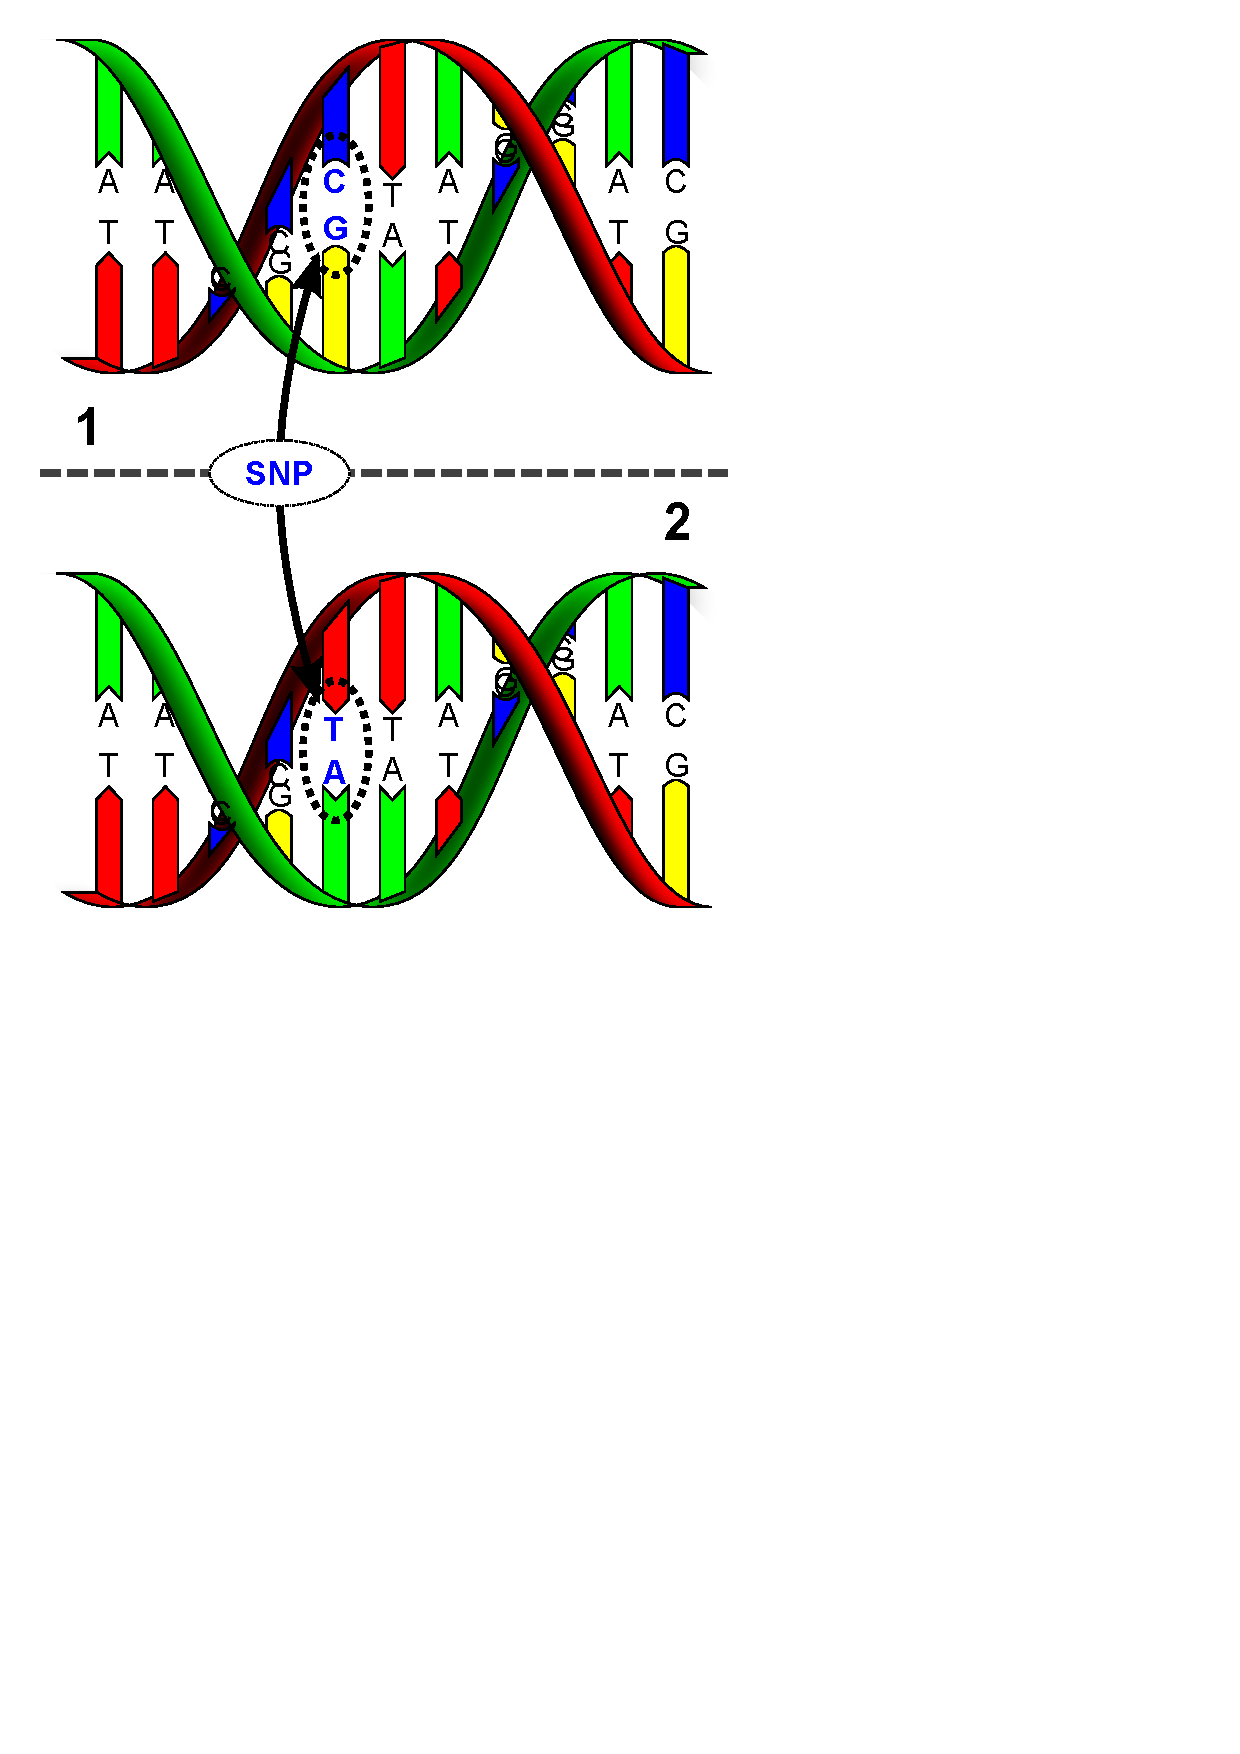
\includegraphics[height=4cm]{SNP}   
    \caption{SNP (wikipedia)}
  \end{figure}
\end{multicols}

\end{frame}


\begin{frame}
  \frametitle{Summarize 500,000 variables in 2}

  \begin{figure}
    \centering
      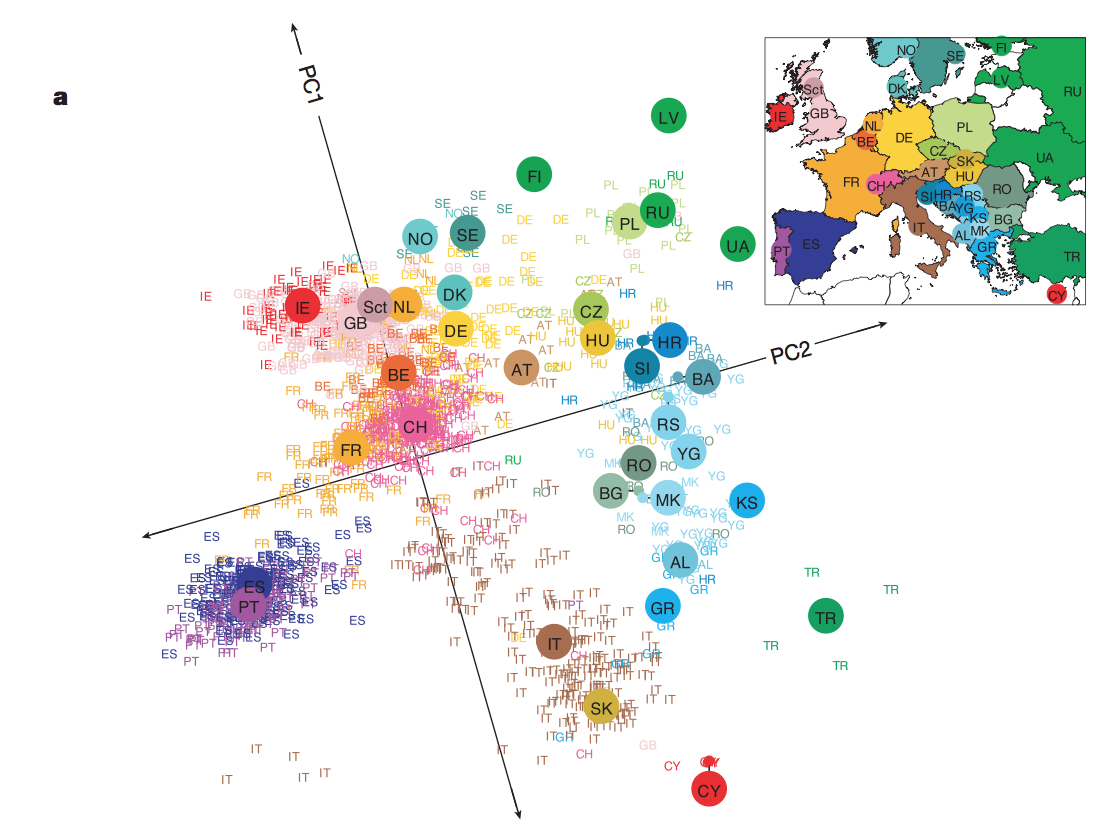
\includegraphics[height=5.5cm]{geneMirrorGeography}
    \caption{PCA output {\tiny source: Nature "Gene  Mirror Geography Within  Europe", 2008}}
  \end{figure}

  In the original messy $3,000 \times 500,000$ table, we may find
    \begin{itemize}
      \item an extremely strong structure between individuals (\alert{\bf clustering})
      \item a very simple subspace where it is obvious (\alert{\bf dimension reduction})
    \end{itemize}

\end{frame}

\begin{frame}
	\frametitle{Overview of Statistics \& Machine Learning}

	\begin{center}
		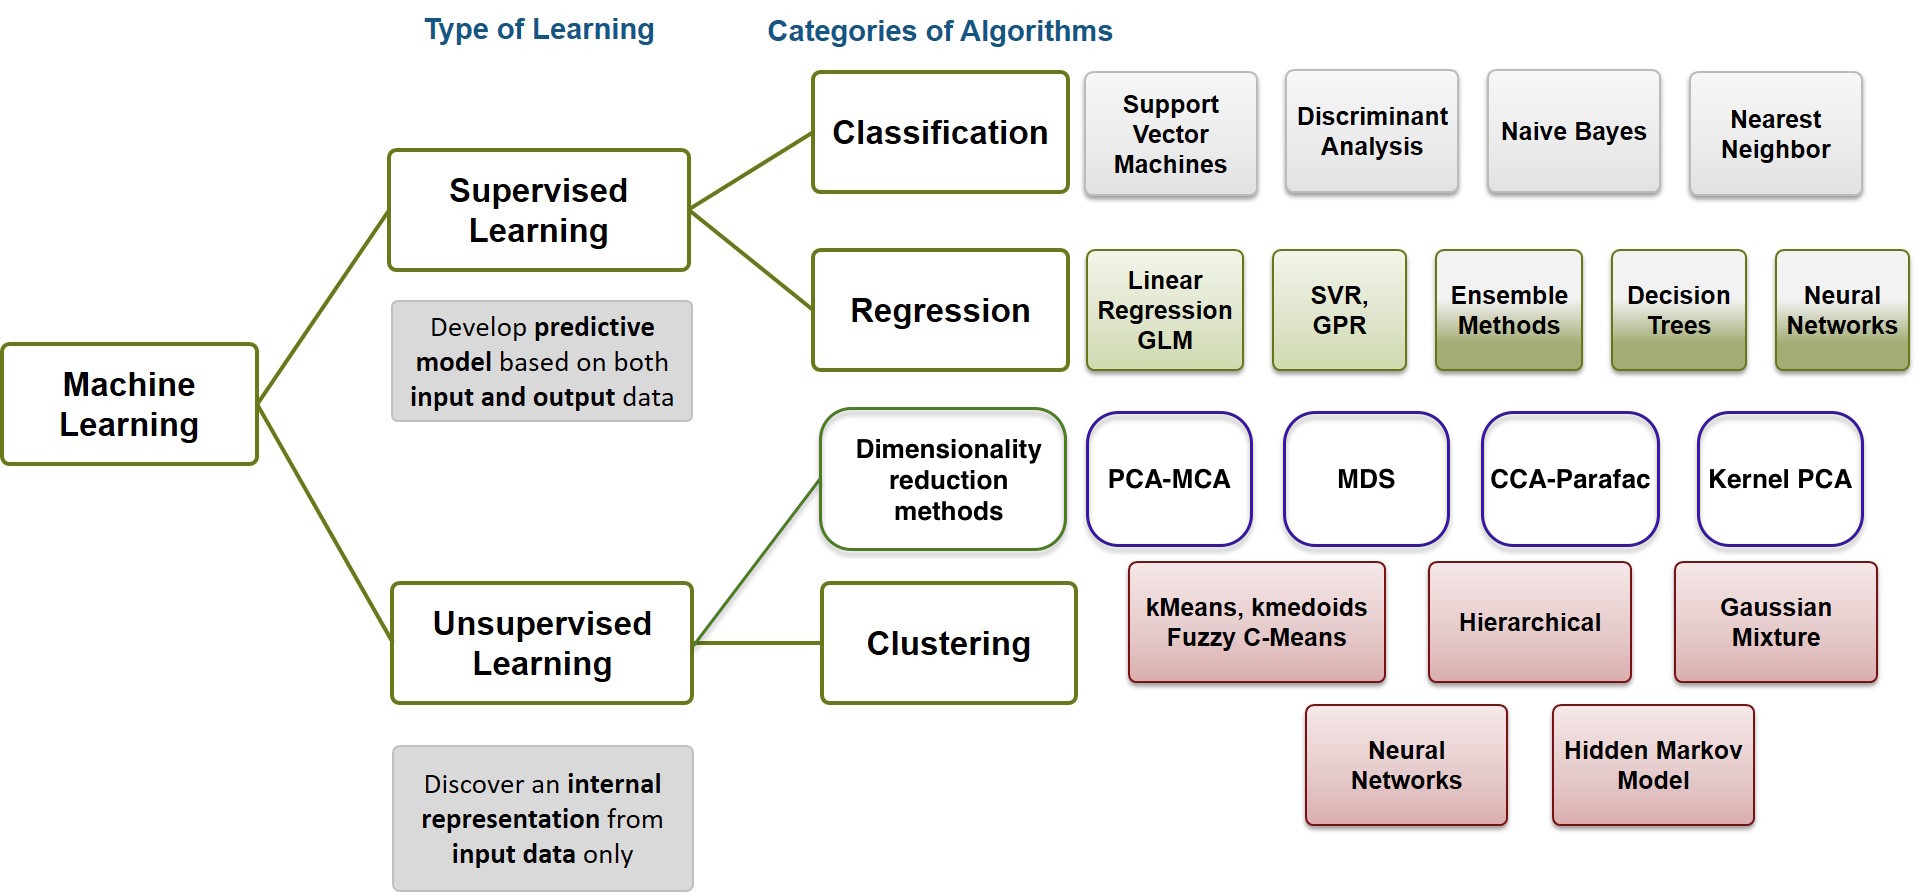
\includegraphics[width=\textwidth]{figures/Learning+Types.jpg}
	\end{center}

\end{frame}

\begin{frame}
  \frametitle{Supervised vs Unsupervised Learning}

  \onslide<1>{  
  \begin{block}{Supervised Learning}
    \begin{itemize}
    \item Training data $\mathcal{D}_n = \{(\bx_1, y_1), \ldots, (\bx_n, y_n)\}, X_i \sim^{\text{i.i.d}} \mathbb{P}$
    \item Construct a predictor $\hat f : \mathcal{X} \rightarrow \mathcal{Y}$ using $\mathcal{D}_n$
    \item Loss $\ell(y, f(x))$ measures how well $f(x)$ predicts $y$
    \item Aim: minimize the generalization error
    \item Task: Regression, Classification
    \end{itemize}
    $\rightsquigarrow$ The goal is clear: predict $y$ based on $x$ (regression, classification)
  \end{block}
  }
  
  \onslide<1,2>{  
    \begin{block}{Unsupervised Learning}
    \begin{itemize}
      \item Training data $\mathcal{D} = \{\bx_1, \ldots, \bx_n\}$
      \item Loss? , Aim?
      \item Task: Dimension reduction, Clustering
    \end{itemize}  
    $\rightsquigarrow$ The goal is less well defined, and \emph{validation} is questionable
  \end{block}
  }
  
\end{frame}

\begin{frame}[label=DimensionReduction]
  \frametitle{Dimension reduction: general goals}

  \paragraph{Main objective:} find a \alert{\bf low-dimensional representation} that captures the "essence" of (high-dimensional) data

  \vfill

  \begin{block}{Application in Machine Learning}
  Preprocessing, Regularization
  \begin{itemize}
    \item compression, denoising,  anomaly detection
    \item Reduce overfitting in supervised learning (improve performances)
  \end{itemize}
  \end{block}

\vfill

  \begin{block}{Application in statistics and data analysis}
    Better understanding of the data 
    \begin{itemize}
      \item descriptive/exploratory methods
      \item visualization: difficult to plot and interpret $> 3d$!
    \end{itemize}
  \end{block}

\end{frame}

\begin{frame}[label=Clustering]
  \frametitle{Clustering: general goals}

  \paragraph{Main objective}: construct a map $f$ from $\mathcal{D}$ to $\{1,\ldots,K\}$ where $K$ is a fixed number of clusters.
    
  \vfill
    
  \paragraph{Careful! classification $\neq$ clustering}
      \begin{itemize}
      \item Classification presupposes the existence of classes
      \item Clustering labels only elements of the dataset
      \begin{itemize}
      \item[$\rightsquigarrow$] no ground truth (no given labels)
      \item[$\rightsquigarrow$] discovers a structure "natural" to the data
      \item[$\rightsquigarrow$] not necessarily related to a known classification
      \end{itemize}
      \end{itemize}
  
  \vfill

  \paragraph{Motivations}
    \begin{itemize}
    \item describe large masses of data in a simplified way,
    \item structure a set of knowledge,
    \item reveal structures, hidden causes,
    \item use of the groups in further processing, 
    \item \dots
  \end{itemize}

\end{frame}


\begin{frame}
  \frametitle{Goals of MAP573}

  \begin{block}{Comprehensive introduction to unsupervised learning}  
    \begin{itemize}  
      \item Dimension Reduction
      \item Clustering
      \item + handling missing data
    \end{itemize}
  \end{block}

  \vfill
  
  \begin{block}{Practical skills for data/exploratory analysis}
      \begin{itemize}  
        \item by applying classical unsupervised approaches and their recents developments
        \item by performing complete analyses via projects
        \item To develop critical evaluation
      \end{itemize}
  \end{block}

\end{frame}

\begin{frame}
  \frametitle{Outline}
  
  \begin{block}{Part 1: 2 sessions to get started with \C{R}}
    $\rightsquigarrow$ 2 lectures set of tutorials, 2 homework assignments
  \end{block}

  \vfill

  \begin{block}{Part 2: 4 sessions on dimension reduction and clustering}
    $\rightsquigarrow$ 4 lectures, 2 tutorials, 2 labs, 4 homework assignments
  \end{block}

  \vfill

  \begin{block}{Part 3: Projects follow-up}
    $\rightsquigarrow$ Apply/develop methods and skills seen in parts 1 and 2 on "real world" data sets
  \end{block}


\end{frame}

\begin{frame}
  \frametitle{Practical information}
  
  \paragraph{Time} -- Tuesday, 1.30pm - 6pm (zoom essentially\dots)

  \vfill

  \paragraph{Team} -- Florian Bourgey / Julien Chiquet / Élise Dumas

  \vfill
  
  \paragraph{Grades}
    \begin{itemize}
      \item  50\% homework (6) \\
      Rmd reports must be submitted during the first 6 weeks
      \item  50\% projects \\
      Report + talk (groups of 4 or 5 people)
    \end{itemize}

  \vfill

  \paragraph{Resources}
    \begin{itemize}
      \item Website \url{https://jchiquet.github.io/MAP573}
      \item Moodle of MAP573 (material, forum, assignments, references)
    \end{itemize}

\end{frame}

\end{document}
